\documentclass[10pt,a4paper]{article}
\usepackage[utf8]{inputenc}
\usepackage{amsmath}
\usepackage{amsfonts}
\usepackage{amssymb}
\usepackage{graphicx}

\usepackage{verbatim}
\usepackage[output-decimal-marker={,}]{siunitx}

\usepackage[left=2cm,right=2cm,top=2cm,bottom=2cm]{geometry}
\author{Adriano del Vincio}
\title{Notes about A1 trasverse asymmetry experiment}
\linespread{1.2}


\begin{document}
\maketitle

\paragraph{}
The aim of these notes is to describe each parts of the analysis of the experiment A1 about the mesurement of the transverse asymmetry. The focus will be on the code of the program used to extract the physical asymmetry and  the data collected by the detectors (from now on called detector A and B): 


\paragraph{Structure of the Event}

Differently from the classic experiment of particle physics, in this experiment an Event is considered the amount of data collected by the two detectors over a temporal window that is \SI{20}{\milli\second} long. The data collected by the two detectors are the counts of scattered electron by a thin target of carbon and lead ($\SI{10}{\milli \meter}$ for carbon and \SI{5}{\milli \meter} for lead). The target respect the convention that his lenght is under $10\%$ of the radiation lenght (to avoid double scattering events). Mami (\textit{Mainzer Microtron}) is an accelerator that produce a continuos beam of electrons that is sent towards two different experiment (A1 and A2 collaborations). The energy at which Mami works for the experiment will be \SI{0.57}{\giga\electronvolt}. The Cross section of the electrons with such amount of energy is dominated by elastic scattering. The physical quantity to measure is the asymmetry between the number of scattered electrons, using incident electrons with two different polarity state ($\uparrow$ and $\downarrow$) transverse polarized with respect to the scattering plane. 

\begin{equation}
asym = \frac{A_{+} - A_{-}}{A_{+} + A_{-}} \text{(expected $\sim$ -20 ppm, Q = \SI{0.2}{\giga\electronvolt c^{-1}})}
\end{equation}

This quantity is computed for each event, that is diveded in 4 different sub-events. The polarity for each event can be of type +,-,-,+ or -,+,+,-, and is produced at the first stage of the accelerator, using circular polarized light to produce the polarized transverse beam. The polarization pattern is randomply selected using a De Bruijn sequence implemented using an arduino (\textit{add photo and explanation}). The percentage of polarization for the beam is roughly $80 \%$, and the recostructed asymmetry should be scaled correctly by this factor. The counts are collected by two detectors, which are made, respectively, of three and nine pmts coupled to a fused silica bar.  


\section{Reconstruct the asymmetry}

It's possible to obtain a raw exstimation of the asymmetry directly taking the average over all the asymmetry computed for each event. However this raw asymmetry needs to be corrected for variations in the beam that affect the measurement. The counts of the pmts can be slightly different due to the variation of the position of the beam on the target, the variations of the incident angles, the uncertain associated with the energy and the current of the beam. All this quantity can influence the asymmetry measured by the pmts, considering also that the expected asymmetry is in the order of ten part per million, and small asymmetry introduced by fluctuations on the beam parameters are not negligible. Correcting the false asymmetries that rise from those uncertainties is a tough task, and it's more easy to adopt a different strategy. Knowing that the beam parameters produced by Mami are quite stable over the time, we can assume a linear model as the following:

\begin{equation}
Asym = A_{physical} \cdot P + \delta_{I} + A_{x} \delta x + A_{y} \delta y + A_{\theta_{x}} \delta \theta_{x} + A_{\theta_{y}} \delta \theta_{y}+ A_{E} \delta E 
\end{equation}

$A_{physical}$ is the aim of the experiment, $A_{x}$ and $A_{y}$ are the asymmetries induced by the variation of the posizion of the beam, $A_{\theta_{x}}$ and $A_{\theta_{y}}$ are the asymmetry associated to angles, $A_{E}$ is the asymmetry associated to the beam energy. 
The relevant assumption is that, for small variation of the beam, the false asymmetry are linearly dependent on the Beam uncertainties (that are $\delta x, \delta y, \delta \theta_{x}, \delta \theta_{y}, delta_{E}$), so a first order approximation seems valid. Collecting all the beam parameters for each sub-event allow the possibility to perform a linear fit to extract the physical asymmetry (the offset) and the false asymmetries.  We will refer to these differences between the sub-events as correlated-differences. 

 

\section{Processing the Data}

The RawData from each monitors are collected by the VFC, and need to be processed to obtain the physical quantity that are important for the analysis. (single and multichannel, synchronous voltage-to-frequency converters (AD7741)) were used for the Beam monitors. Data are obtained in the following way:  an analog input signal is sent to the electronics, from $-V_{ref}$ to $V_{ref}$. The Output signal returned from the electronic is a square waves whose frequency is proportional to the input signal. The output frequency goes from $5\% f_{ref}$ to $45\% f_{ref}$ (with $f_{ref}$ we are indicating the reference frequence of the VFC). For each monitors the measurements are about counting the number of pulses in the output signal, during a period of time that is roughly $20ms$. During the beam time the $f_{ref}$ will be set to $\sim$ \SI{6}{\mega\hertz}, so a period of \SI{20}{ms} correspond to a number of pulses of $\sim 117000$. Following the logic of how the vfc are operating, we can derive the formula to convert the number of pulses that make up the data to the corresponding values in Volt. 

\begin{equation}
V_{measured} = V_{range} ( 2 \dfrac{( N_{out} - 5\% \cdot Period )}{ 40\% \cdot Period} -1)
\end{equation}

The number of output pulses is $N_{out}$, that goes from $5\% \cdot Period$ to $45\% \cdot Period$. 
The obtained values still are not physical values about the beam. We need to convert the Volt in physical quantity, as \si{\micro \meter} or \si{\micro \ampere}. All the voltage values are converted in physical quantity using the following:

\begin{equation}
 V_{phys} = (V_{measured} - offset) \cdot scale 
\end{equation}

all the factors needed for the conversion are obtained from dedicated calibration measurements during the beamtime. For the experiment, there are 11 monitors in total, which will measuere the following quantity:

\begin{itemize}

\item \textbf{I21} and \textbf{I13} to measure the beam current.
\item \textbf{E18} that measure the energy of the beam.
\item \textbf{X21},\textbf{Y21},\textbf{X26},\textbf{Y26},\textbf{X25},\textbf{Y26} to measure the position of the beam in the \textit{xy} plane, with the convenction that the beam is moving in the \textit{z} direction.

\end{itemize}

For the beam line, and also for knowing the exact position of the monitors (needed to compute some values for the fit) it's useful to draw a scheme of the beam line here:

\begin{center}
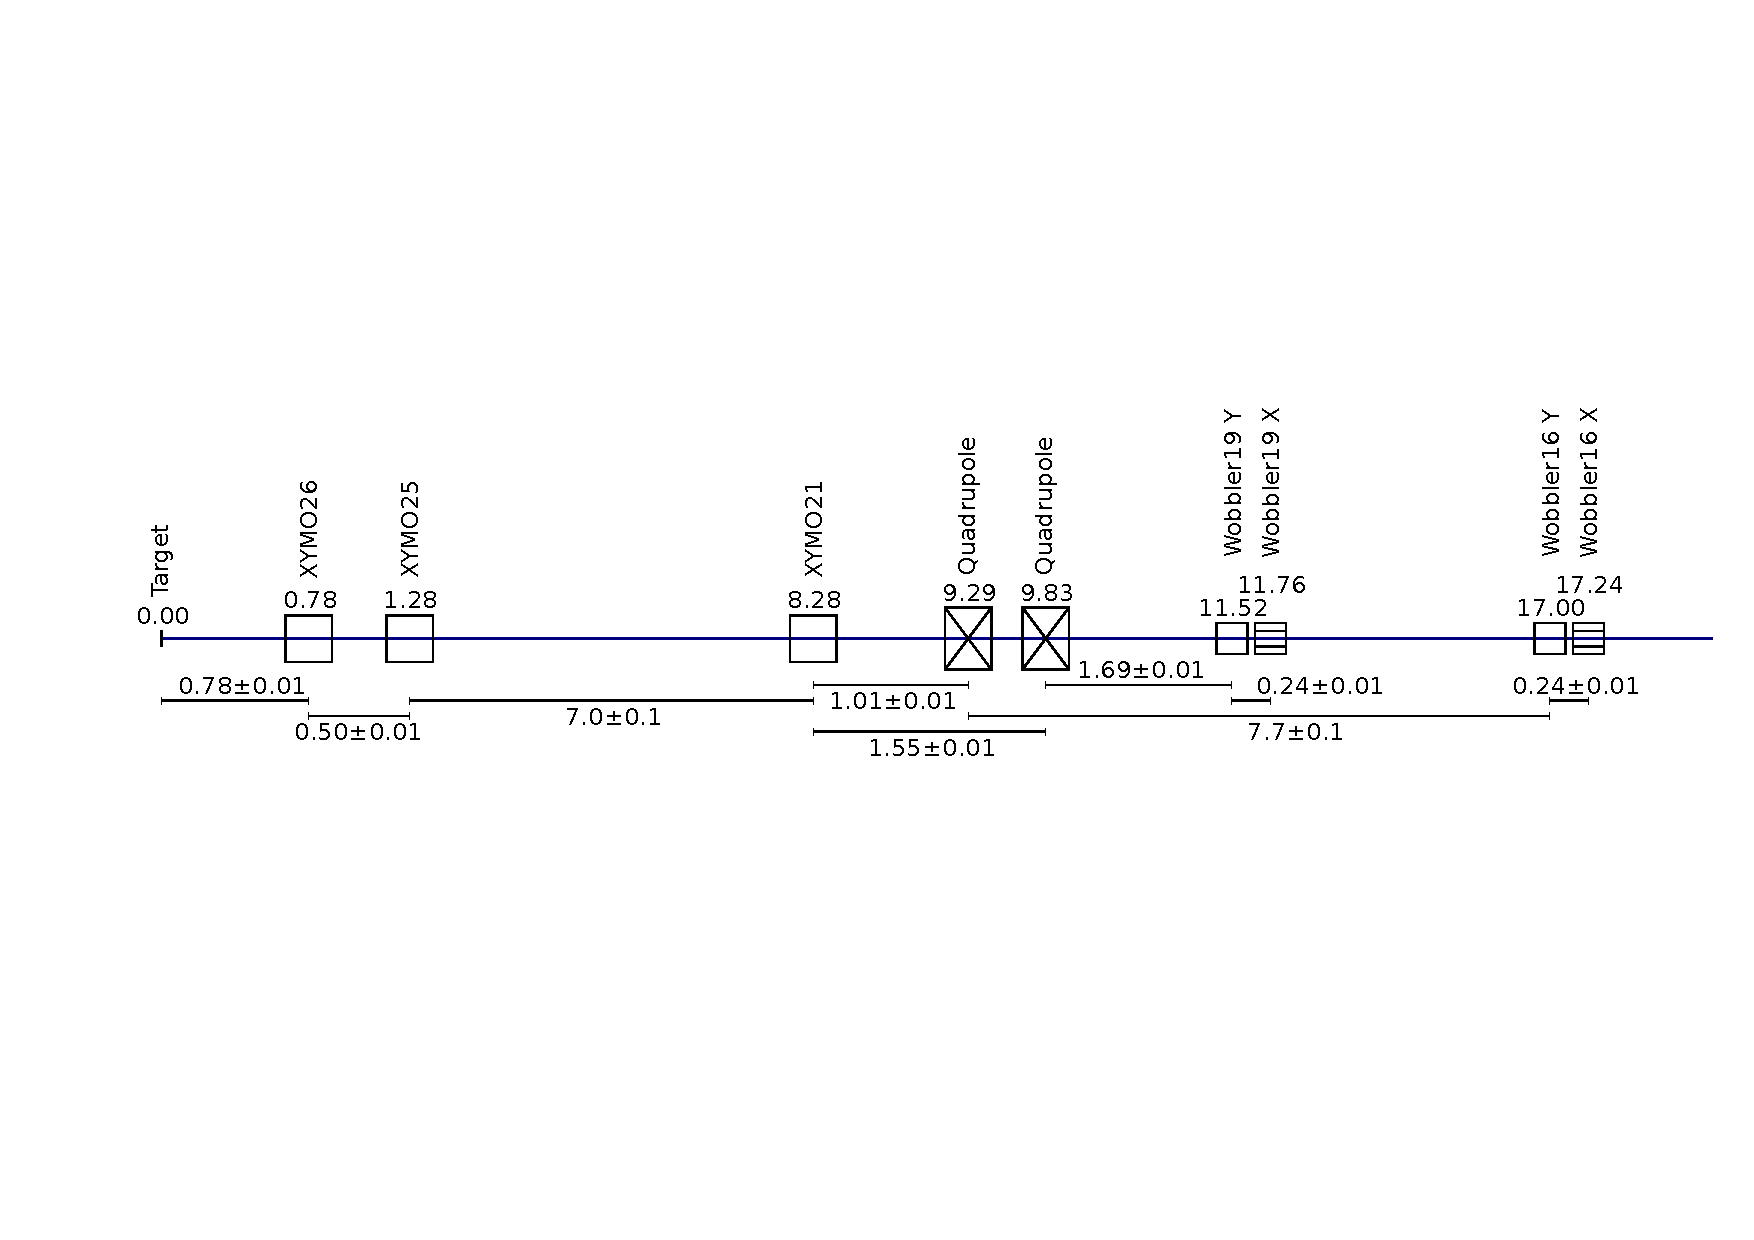
\includegraphics[scale=0.4]{figures/XYMOCalibBeamLine.svg.pdf} 
\end{center}

The position of the \textbf{X/Y} monitors in the figure (given in meters) are needed to compute: 

\begin{itemize}
\item $x_{position}$ on the target
\item $y_{position}$ on the target
\item $\theta_{x}$ scattering x angle
\item $\theta_{y}$ scattering y angle 
\item $E18$ energy of the Beam
\item $I$ Beam current
\end{itemize}

It is possible that those quantity are associated to false asymmetries that need to be corrected to obtain the physical transverse asymmetry we are interested to measure. To be precise the quantities used in the fit will be indicated as hcd, and are computed in a dedicated script of the analysis program, called \textit{Calculation.cc}

\begin{equation}
\delta x =  \frac{(x_{up,1} + x_{up,2})}{2} - \frac{(x_{down,1} + x_{down,2})}{2}
\end{equation}

Where with $1,2$ we are referring to the two sub-events with the same polarization.
What is important to remember is that we are measuring the asymmetry about the number of counts of the spectrometer for different polarized scattered electrons. So the quantity that are more important for the analysis are the correlated-differences (hcd) defined as the average of the difference between the values measured for up-polarized electrons and down-polarized electrons. 

\paragraph{Current asymmety}

One the false asymmetry that needs to be included in the fit is the current asymmetry. It's the simplest false asymmetry to be corrected for the data. This is quite clear starting from the cross section definition:

\begin{equation}
\frac{dN}{dt} = I_{0} n_{t} \frac{\sigma}{S}
\end{equation}

where $I_{0}$ is the beam current, $n_{t}$ is the density of the target, and S is the surface of the beam. With this we can directly compute the asymmetry:

\begin{equation}
Asym = \dfrac{\frac{dN_{\uparrow}}{dt} - \frac{dN_{\downarrow}}{dt}}{\frac{dN_{\uparrow}}{dt} + \frac{dN_{\downarrow}}{dt}} = \dfrac{\sigma_{\uparrow} I_{0 \uparrow} - \sigma_{\downarrow} I_{0 \downarrow}}{\sigma_{\uparrow} I_{0 \uparrow} + \sigma_{\downarrow} I_{0 \downarrow}}
\end{equation}

Considering that the cross section slightly change for up/down polarization, to correct the current asymmetry we need:

\begin{align*}
Asym - \dfrac{I_{0 \uparrow} - I_{0 \downarrow}}{I_{0 \uparrow} + I_{0 \downarrow}}
\end{align*}

this is a consequence of the fact that the luminosity is proportional to the beam current, so we don't need to add a new parameter to the model.

\paragraph{Energy correlated-difference}

The energy of the Beam directly change the cross-section, so the number of counts of the detectors. If there is a systematic change in energy from up to down polarized electrons, the asymmetry measured for each event can be different from what we expect. 

\paragraph{Position}
The position of the beam on the target is computed cosidering that the particle are following a linear motion toward the target, so we describe the particles with the simply equation: $y = mx + q$. By imposing the passage of the particles at the y26, y25 and x26,x25 coordinates, we can obatin the hitting positions on the target. In our convenction, the origin of the coordinate system overlap with the position of the target, so we need to compute the offeset $q$. It's quite simple to show that the formula are:

\begin{equation}
q_{x} = \dfrac{X25 Z21 - X21 Z25}{Z21 - Z25}
\end{equation}

\begin{equation}
q_{y} = \dfrac{Y25 Z21 - Y21 Z25}{Z21 - Z25}
\end{equation}

Those data are stored in the data-tree. For each sub-events the position qx e qy is calculated, and it's stored in an array. An interesting details about the position of the beam on the target is that it will change during the data acquisition with lead, to prevent the target from melting.

\paragraph{Angle}
The angle useful for the analysis are the $\Theta_{x}$ and $\Theta_{y}$ angles on the target. These quantities are calculated with the following formula:

\begin{equation}
\Theta_{x,y} = \dfrac{(X/Y)_{25} +  (X/Y)_{21}}{ Z_{25} - Z_{21}} 
\end{equation}

with $Z_{25}$ and $Z_{21}$ the position of the two monitors in the beam line. This formula is obtained, also in this case, considering a linear motion and using the fact that the agles are supposed to be very small (so we can approximate the tangent to the first order).

\paragraph{pmts Counts}

The pmts counts are analyzed separately, using two different trees for handling the data: spekA and spekB. Because the two spektrometers (where our detectors will be placed) are allocated in different direction respect to the beam line, they will measure asymmetries with different signs. For each pmts that composes the spectrometer, there will be 4 different thresholds, selected with the Data acquisition board. The rawCounts are loaded from from the data files and stored in the data tree. As for the other monitors, in \textit{Calculation.cc} a function calculates the offsetCorrectedCounts, loading from the file \textit{standard.conf} the offsets of each pmt and then subtracting it from the rawCounts. Other values that are defined and computed are the Asymmetry, which doesn't need ad explanation, and the PolarityCorrelatedDifference and the rawIntraEventDifference, that are defined as:


\begin{gather*}
 pcd = \dfrac{Counts_{1,\uparrow} + Counts_{2,\uparrow} - Counts_{1,\downarrow} - Counts_{2,\downarrow}}{2} \\
 ied = \max (Counts_{\uparrow}) - \min (Counts_{\downarrow})
\end{gather*}

These quantities are defined as the average of the difference between the counts of up and down polarized sub-events and the maximum intra event difference, and will be used to check if there are unexpected behaviors in the data (neglecting the true and all the false asymmetries, we are supposed to see roughly the same number of counts for each of the sub-events) and cut out undesidered events from the analysis). 
For the beam time four different threshold for each pmt will be selected and analyzed separately. This will lead, for detercot B, to $12$ different measure of the recostructed asymmetry. The values will be averaged using the following formula:

\begin{align*}
	\dfrac{\sum_{i = 0}^{N_{detectorB/a}} \frac{A_{i}}{\sigma_{i}^{2}}}{\sum_{i = 0}^{N_{spekb/a}} \frac{1}{\sigma_{i}^{2}}}
\end{align*}

Now a scheme to summarize all the quantity that are computed and stored in the data tree, for the experiment: \newpage

\begin{figure}[!hbtp]
\centering
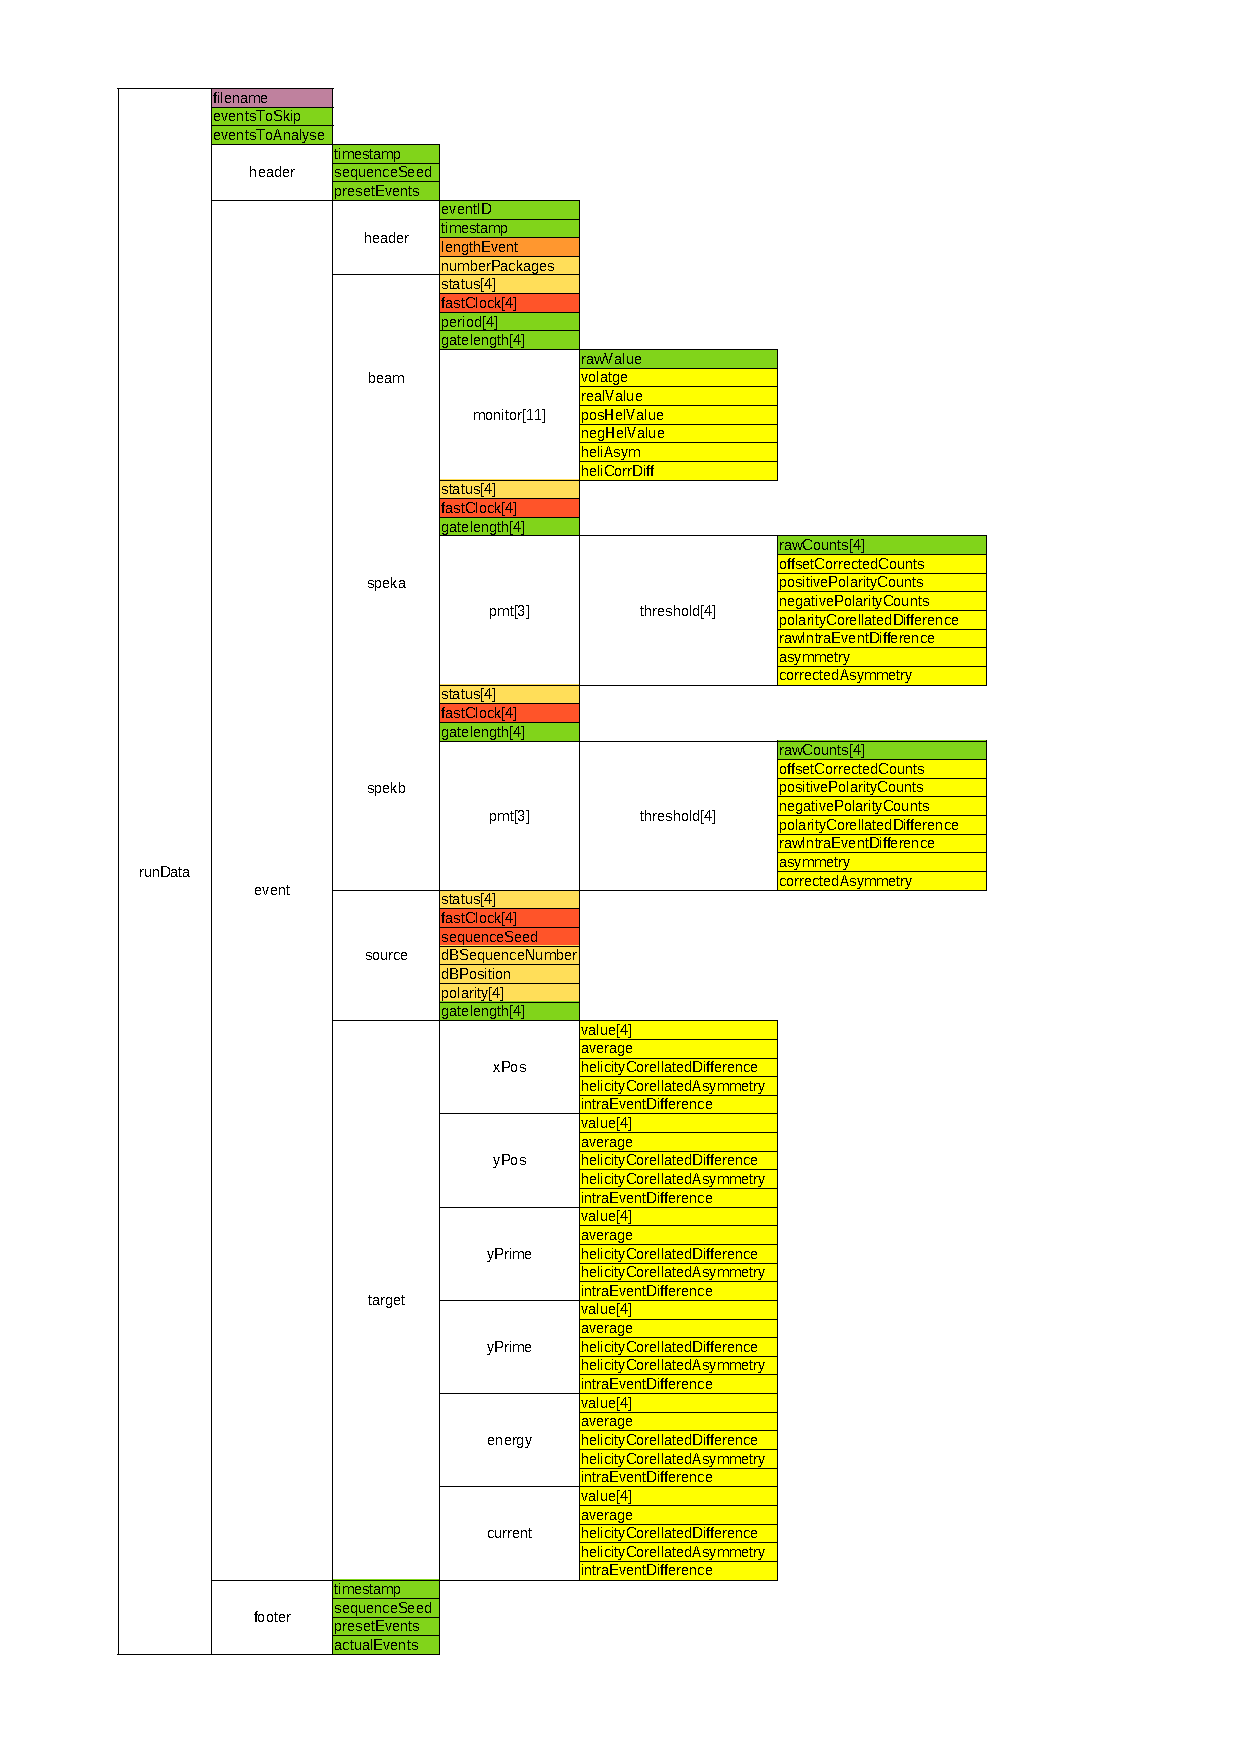
\includegraphics[scale= 0.7]{figures/RunDataStructure.pdf}
\caption{Scheme of the Data Tree}
\label{Data-tree}
\end{figure}


\section{Electronic testing}

For the next Beam time, the primary goal of the experiment is the evaluation of the electronics, that will be tested during the measure of the transverse asymmetry with carbon. The beam time is scheduled for the week (28/11 - 4/12) the electronics for the data acquisition needs to be tested, and also the correct settings for thresholds and voltage supply of the pmts needs to be set properly. At the beginning of the next beam time some operations are needed, before taking data for the transverse asymmetry.  It will be necessary to take pmts counts with different beam current, to check if the behaviour of the pmts is linear with the thresholds and the attenuation setted, and align the two spektrometers to the elastic scattering plane. Before the beam time, it is possible to study the counts of the pmts using cosmic rays, for selecting good values for thresholds, attenuation and power supply.

The number of events expected considering the size of the fused-silica coupled to the pmts (the detection part of the spektrometer B) is roughly $\SI{1}{ \per \minute \per \cm}$. So the expected number of Counts, considering $\SI{10}{ \centi \meter } \cdot \SI{7}{ \centi \meter }$, is around 70 events, that produce Cherenkov light, collected by the dynodes of the pmts. 

\paragraph{NINO board}
The Nino board is the device that is able to collect the number of pulses directly from the pmts. It's made by discriminators which compare the input signals (on the left side) to a signal that can be adjusted manually with the \textit{pvDaq.py} scripts. For spekb the data acquisition is already available and is used to test the pmts, finding the good operation point. Here we display a photo of the Nino board (on the right side the connectors to the pmts of spekB):

\begin{figure}[hbtp]
\centering
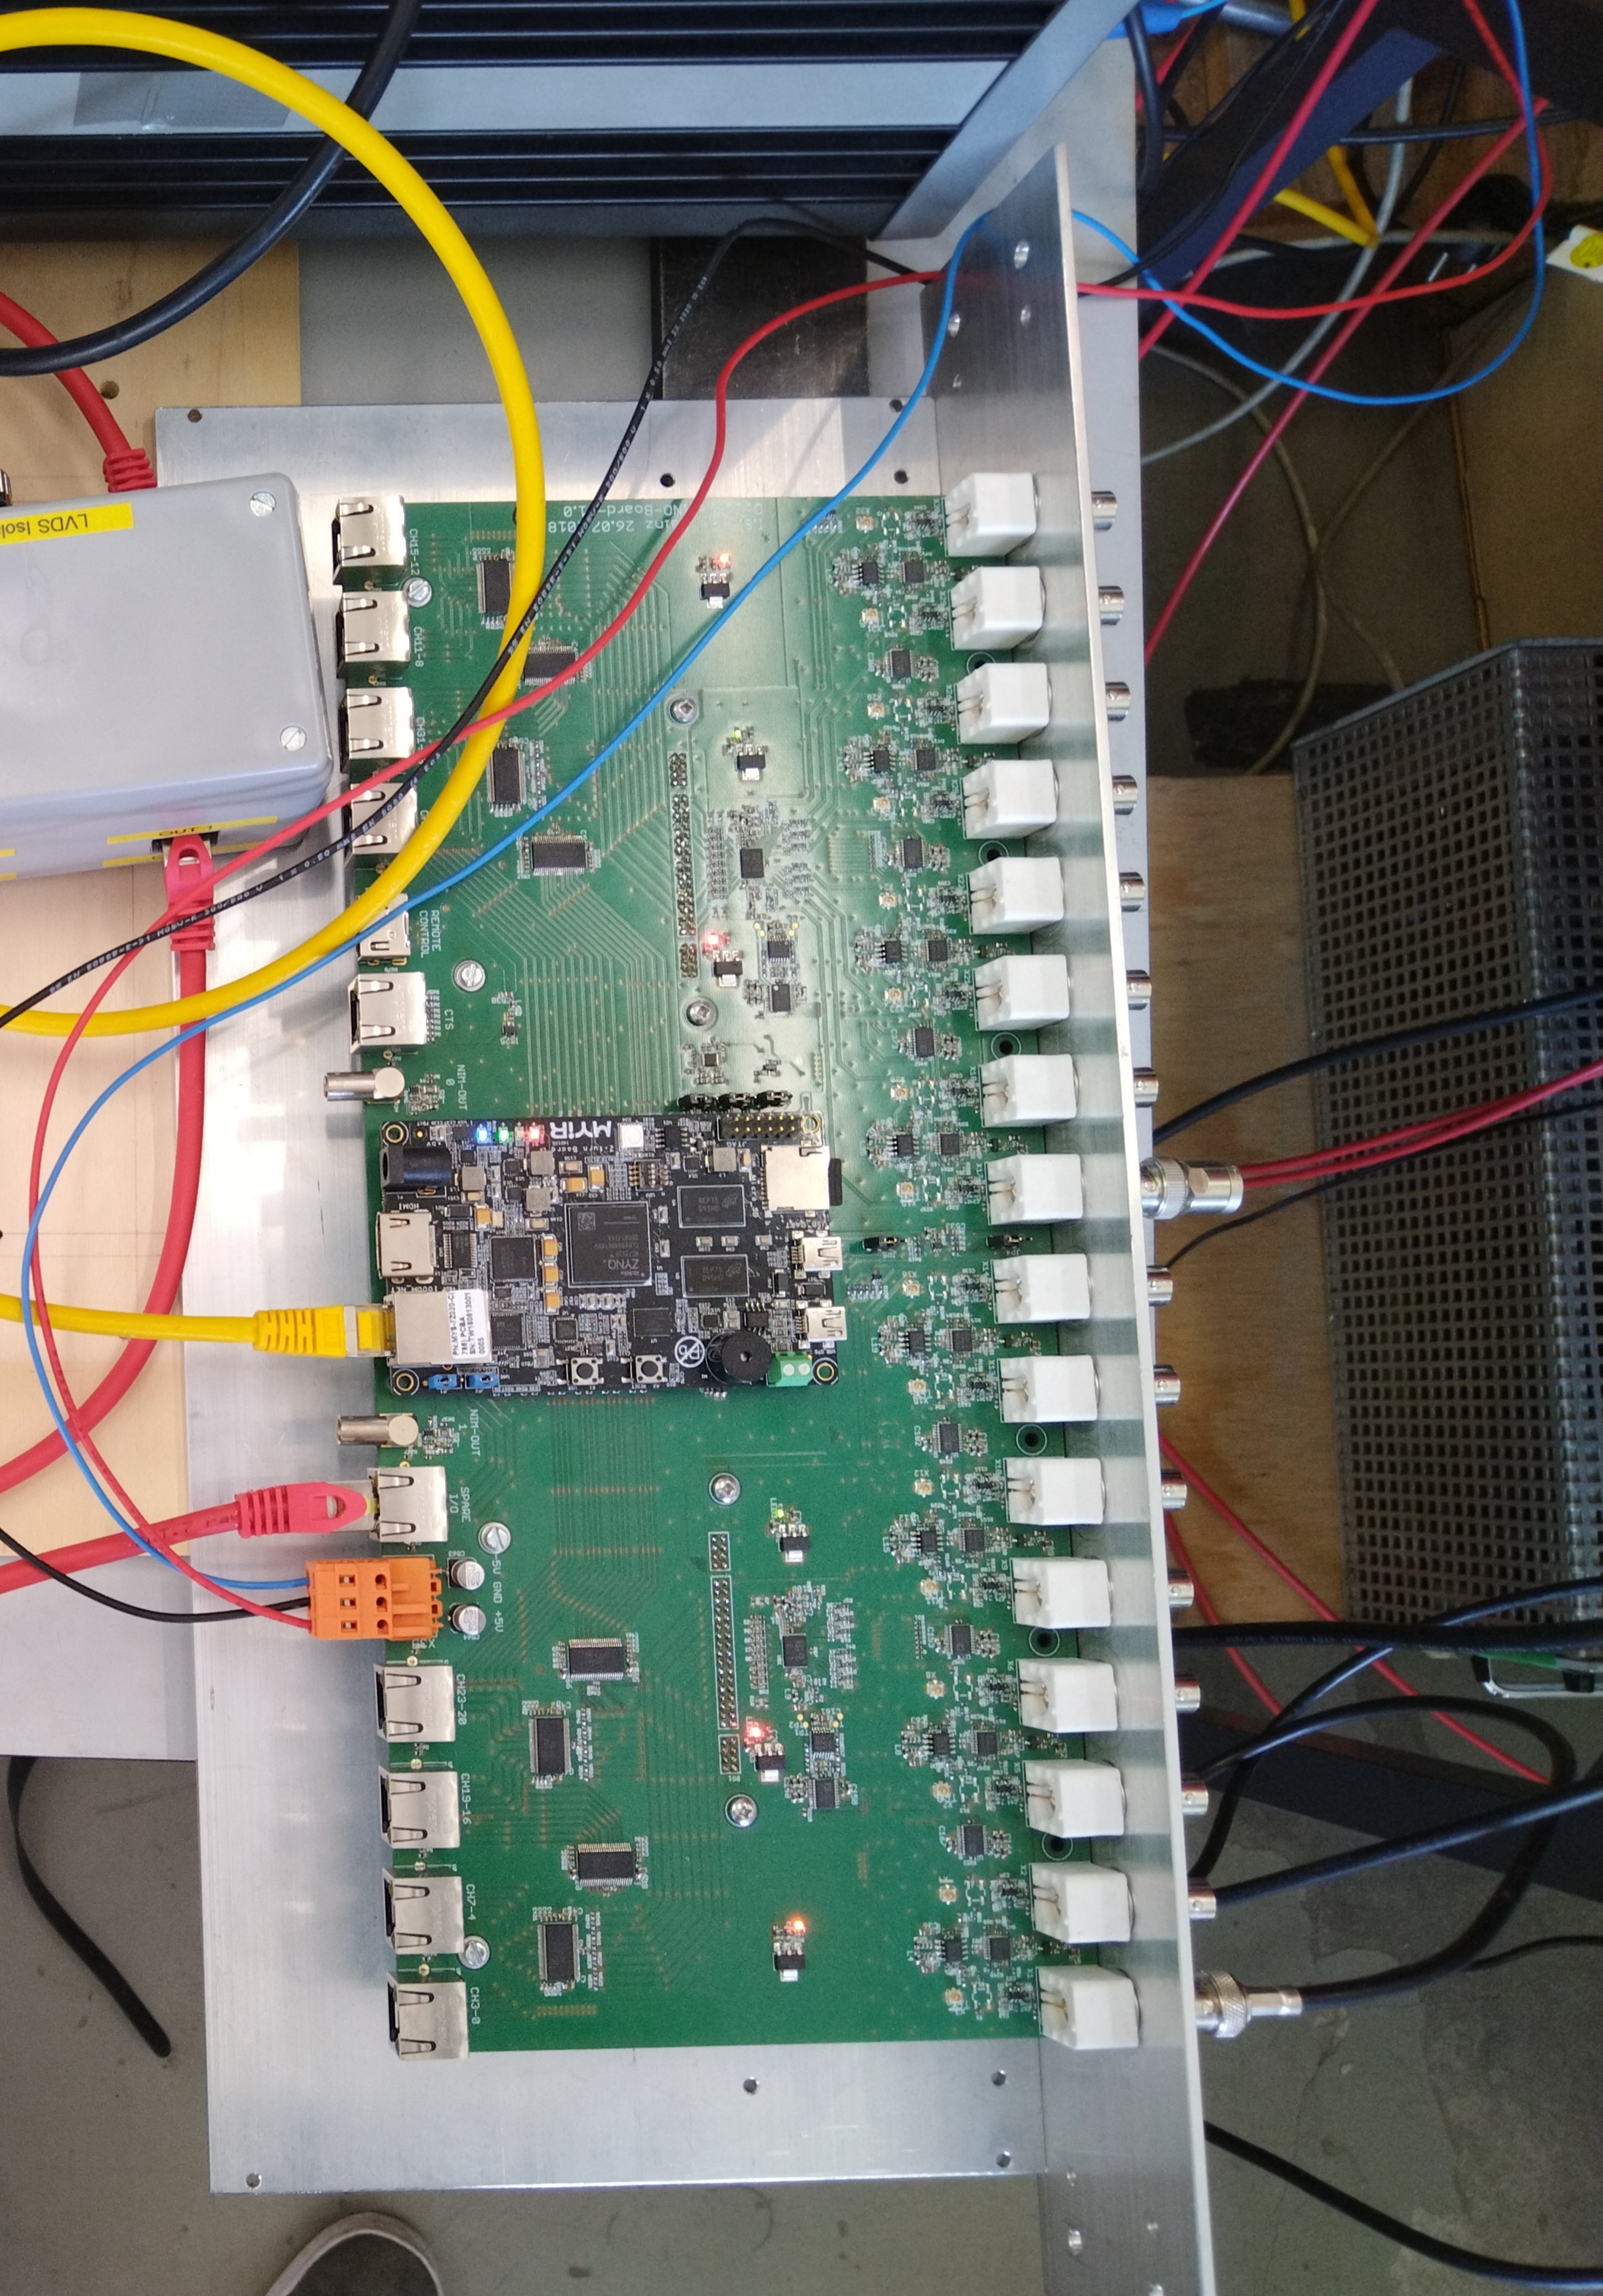
\includegraphics[scale=0.08]{figures/IMG_20221102_193754.jpg}
\caption{Nino board to read-out the input signals}
\end{figure}

For the Nino board there are two different parameters that can be adjusted: Threshold and Attenuation. The Threshold was set to a value equal to 600 for each of the three pmts of the spekb (following the instructions in the documentation), and we just changed the attenuation factor, to change the effective threshold of the pmts. It's important to notice that the Nino board is made in such a way that it doesn't compare to voltage signals, but read the total charge accumulated by the pulse and confront it with an internal threshold that can be changed. So it's not simple to identify a effective threshold in terms of voltage of the input signal. However the behaviour of the Nino board was studies before for the case of counting pulses from a scintillator detector, setting the threshold value at 750 (similar to our setting 600) and changing the attenuation. In this case a voltage threshold is shown, versus the attenuation: 

\begin{figure}[hbtp]
\centering
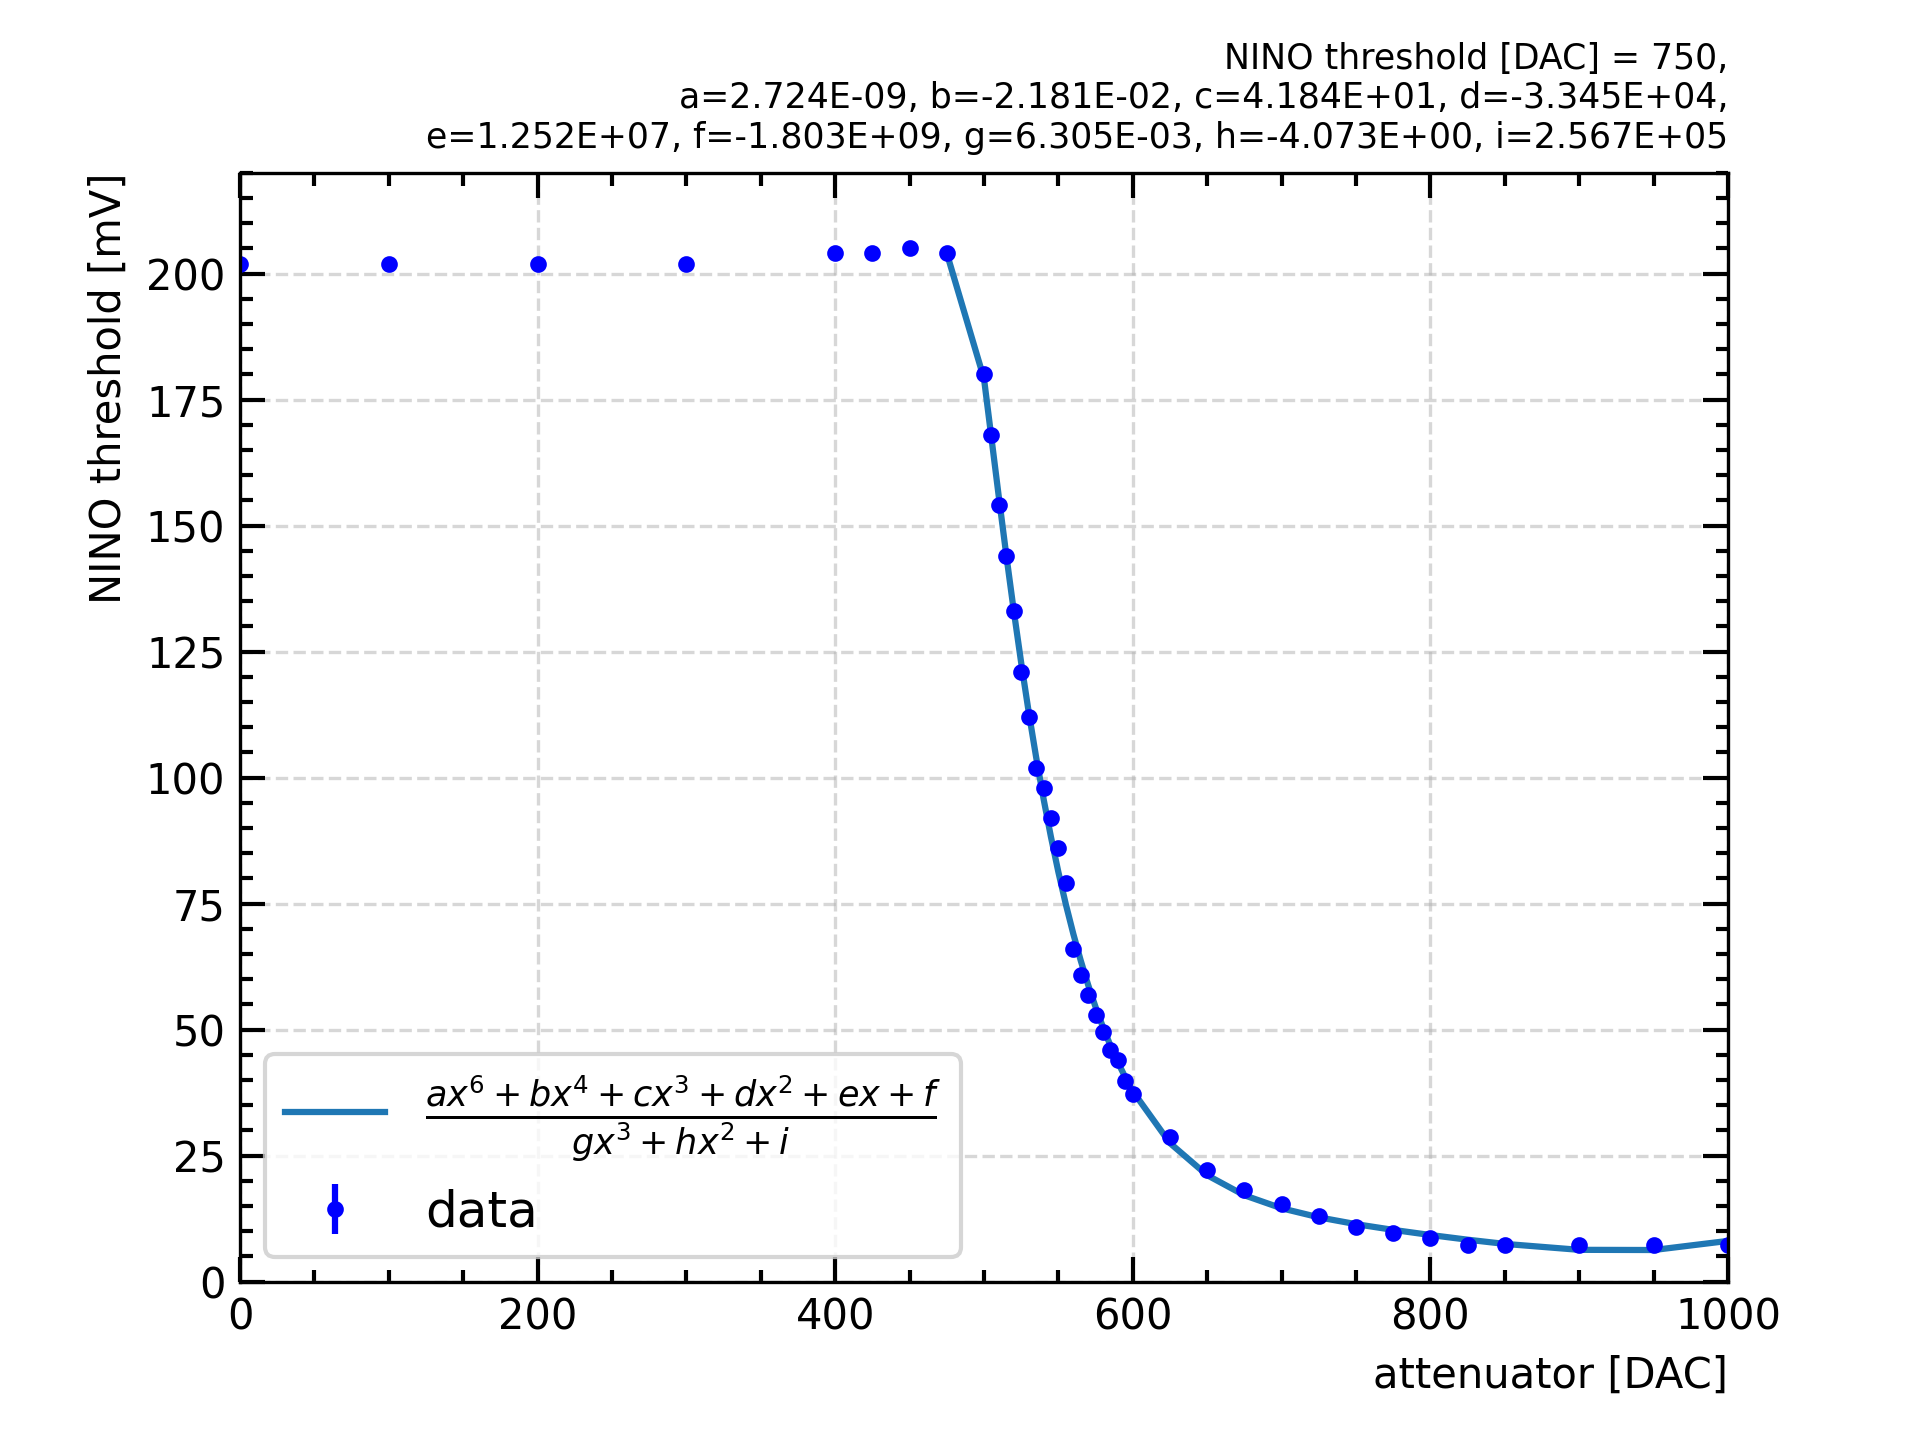
\includegraphics[scale= 0.8]{figures/calibrationCurve_mVRange200.png}
\caption{Calibration curve of the Nino board}
\label{fig:Calibration}
\end{figure}

It's important to remind that our conditions are slightly different: we are using a Cherenkov detector instead of a scintillator (different shape of the pulse) and a different value of the threshold. However this plot give us an indication of the trend of the threshold as a function of the attenuation. From the plot we see that around $500/600$ there is a big variation in the NINO threshold, so the best working point for the pmts is around this values of the attenuation.

\paragraph{Studying the pmts}
The pmts of the spekB are powered with a negative voltage around $\simeq \SI{-900}{\volt}$. Before taking the data we tried to observe some pulses at the oscilloscope, to check if the range of the power supply was correct :

\begin{figure}[hbtp]
\begin{minipage}[b]{0.45\textwidth}
\centering
\includegraphics[width=\textwidth]{figures/IMG_20221027_170925.jpg}
\caption{Signals of the three pmts of spekB observed at the oscilloscope, (threshold 10mV, CH1, CH2 CH3 are pmt 1,2,3)}
\end{minipage}
\begin{minipage}[b]{0.45\textwidth}
\centering
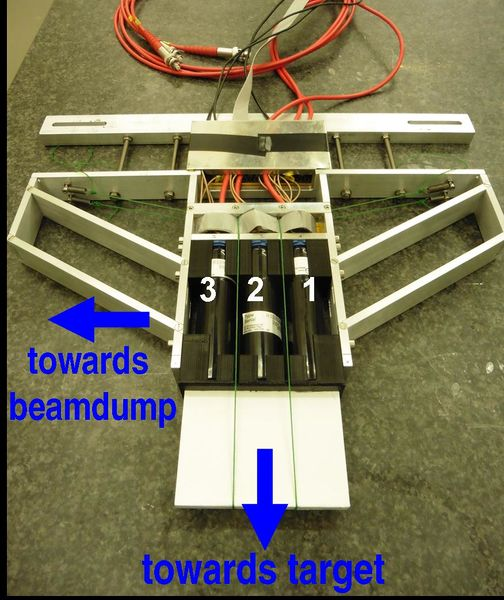
\includegraphics[width = 0.8\textwidth]{figures/504px-Blackfalcon.jpg}
\caption{Spektrometer B }
\end{minipage}
\end{figure}

Then we started taking data varying the attenuation of the NINO board, with threshold fixed at 600. We decided to take a run on $\SI{1}{\minute}$ for some values of the attenuation, ranging from $300$ to $3000$ (maximum values is around $4000$). Our interested is to select a region where the number ot counts are scaling linarly with the attenuation and to identify the region where the behaviour for the pmts is no more linear (noise region). We obserded a small knee in the plot, around the zone of $580-600$ of attenuation, where the number of counts was almost costant, roughly equal to the number of expected events from muons hitting the detector. Reminding the figure (\ref{fig:Calibration}), the threshold, around $500-600$ of attenuation, has the correct value to let the NINO board to collect the pulses produced by the muons.

\begin{figure}[hbtp]
\centering
\begin{minipage}[b]{0.45\textwidth}
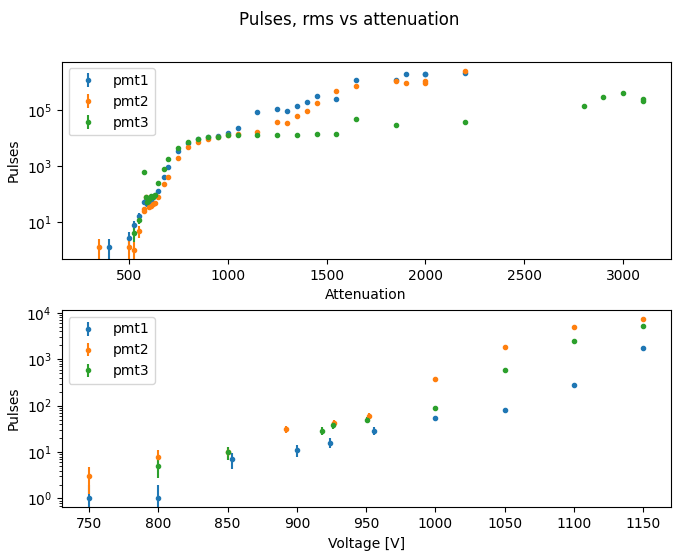
\includegraphics[width=\textwidth]{figures/Attenuation(good).png}
\end{minipage}
\begin{minipage}[b]{0.45\textwidth}
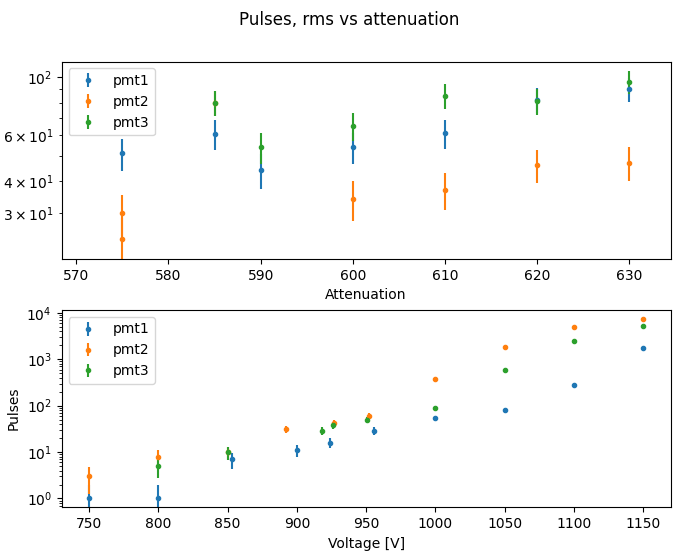
\includegraphics[width=\textwidth]{figures/around 580-630.png} 
\end{minipage}
\caption{Counts of the NINO board versus attenuation (on the top) and voltage (below). On the left is possible to distinguish two different areas, one under $\simeq 750$ attenuation where there is linearity, and a zone on the left where the attenuation is too high and the noise is predominant.}
\label{fig:Attenuation}
\end{figure}


Therefore, we decided to fix the attenuations of the pmt at $600$. 
As we can observe from the plot on the right of figure \ref{fig:Attenuation} the pmt 1 and 3 have roughly the same number of counts. To equalize the behaviour of the three pmts, the power supply of the the second pmt was increased to have the same number of counts. At the end the power supply was fixed to $ \SI{-951}{\volt} , \SI{-925}{\volt}, \SI{-918}{\volt} $.

At this point, we used a Pulser, that was able to produce signal with an high rate ($f = \SI{13.17}{\kilo \hertz}$). We plug the pulser directly in one of the input channenl of the NINO board, and took a run of \SI{1}{\minute} log, to test how good the Daq is in counting the events. For a minute of run, considering that each sub-event last for $\SI{20}{\milli \second}$, we expect $750$ events and $3000$ sub-events. So the expected number of pulses for each event is:

\begin{align*}
\frac{\SI{60}{\second} \cdot f}{4 \cdot 750} = 263.4 
\end{align*}

The values that we obtained analyzing the run and taking the average counts, as shown in the following plot, is different, about the $75\%$ of the number of counts expected. After some investigation we found that the problem was due to a wrong implementation on the fpga program in the Daq, that was resolved. 

\begin{figure}[hbtp]
\centering
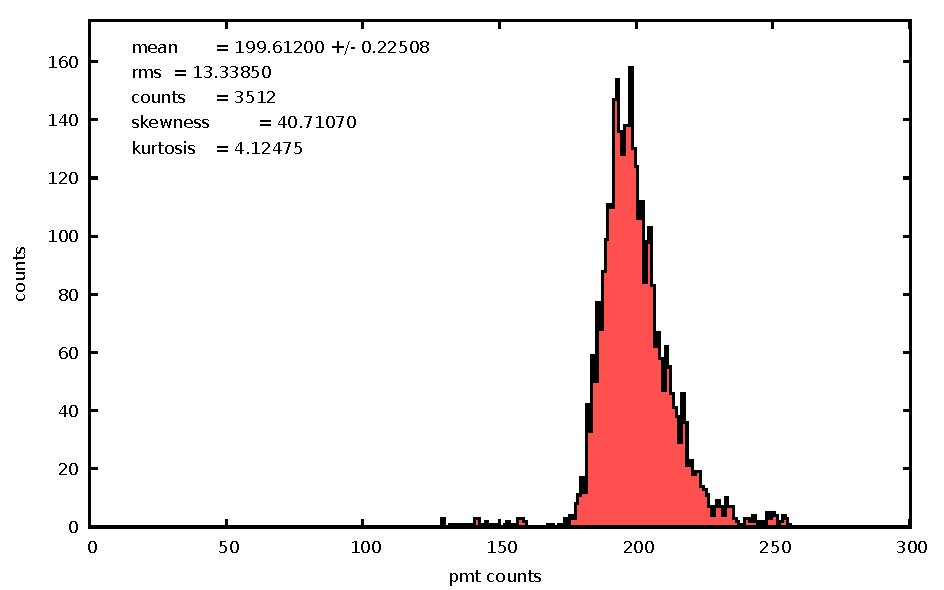
\includegraphics[width=0.5\textwidth]{figures/pmtB.pdf}
\caption{Counts of pmt 1 with the pulser}
\end{figure}

At this point we collected 10 runs, each of them $\SI{1}{\minute}$ long, to study the statistical fluctuation of  the counts: we report here the obtained values:

\begin{center}
\begin{tabular}{|c|c|c|c|}
\hline 
Pmt: & 1 & 2 & 3 \\ 

1 & 58 & 60 & 62 \\ 
\hline 
2 & 62 & 55 & 59 \\ 
\hline 
3 & 61 & 59 & 70 \\ 
\hline 
4 & 73 & 66 & 70 \\ 
\hline 
5 & 68 & 66 & 56 \\ 
\hline 
6 & 59 & 52 & 64 \\ 
\hline 
7 & 69 & 74 & 77 \\ 
\hline 
8 & 48 & 49 & 57  \\ 
\hline 
9 & 70 & 54 & 58 \\ 
\hline 
10 & 60 & 61 & 66\\
\hline
\end{tabular} 

\end{center}

This data are interesting to check if the counts are following the theoretical distribution of the events expected for cosmic rays at sea level. We know that the number of counts should be Poisson-distributed, following:

\begin{equation}
Pdf(\mu,k) =  \frac{\mu^{k}}{k!} e^{-\mu}
\end{equation}

The variance of the poisson distribution is equal to the mean of the counts, and we expect the same behaviour also for the sample mean and the sample variance:

\begin{align*}
\begin{split}
\mu_{1} = 62.8	\qquad \sigma^{2}_{1} = 54.40 \qquad r_{12} = 0.66\\
\mu_{2} = 59.6	\qquad \sigma^{2}_{2} = 57.15 \qquad r_{23} = 0.65\\
\mu_{3} = 63.9	\qquad \sigma^{2}_{3} = 46.98 \qquad r_{13} = 0.35 \\
\end{split}
\end{align*}

The third pmt has a variance lower than the expected, however the correlation between the nearby pmts is of quite high. Besides this, the correlation between the pmt 1 and 2, which are separated, is lower than the correlation between to adjacent pmts. \newline
To check the correct operation of the detector, we exploited the possibility to observe coincidence using  another pmt coupled to a plastic scintillator, placed above the detection area of the detector B:

\begin{figure}[hbtp]
\centering
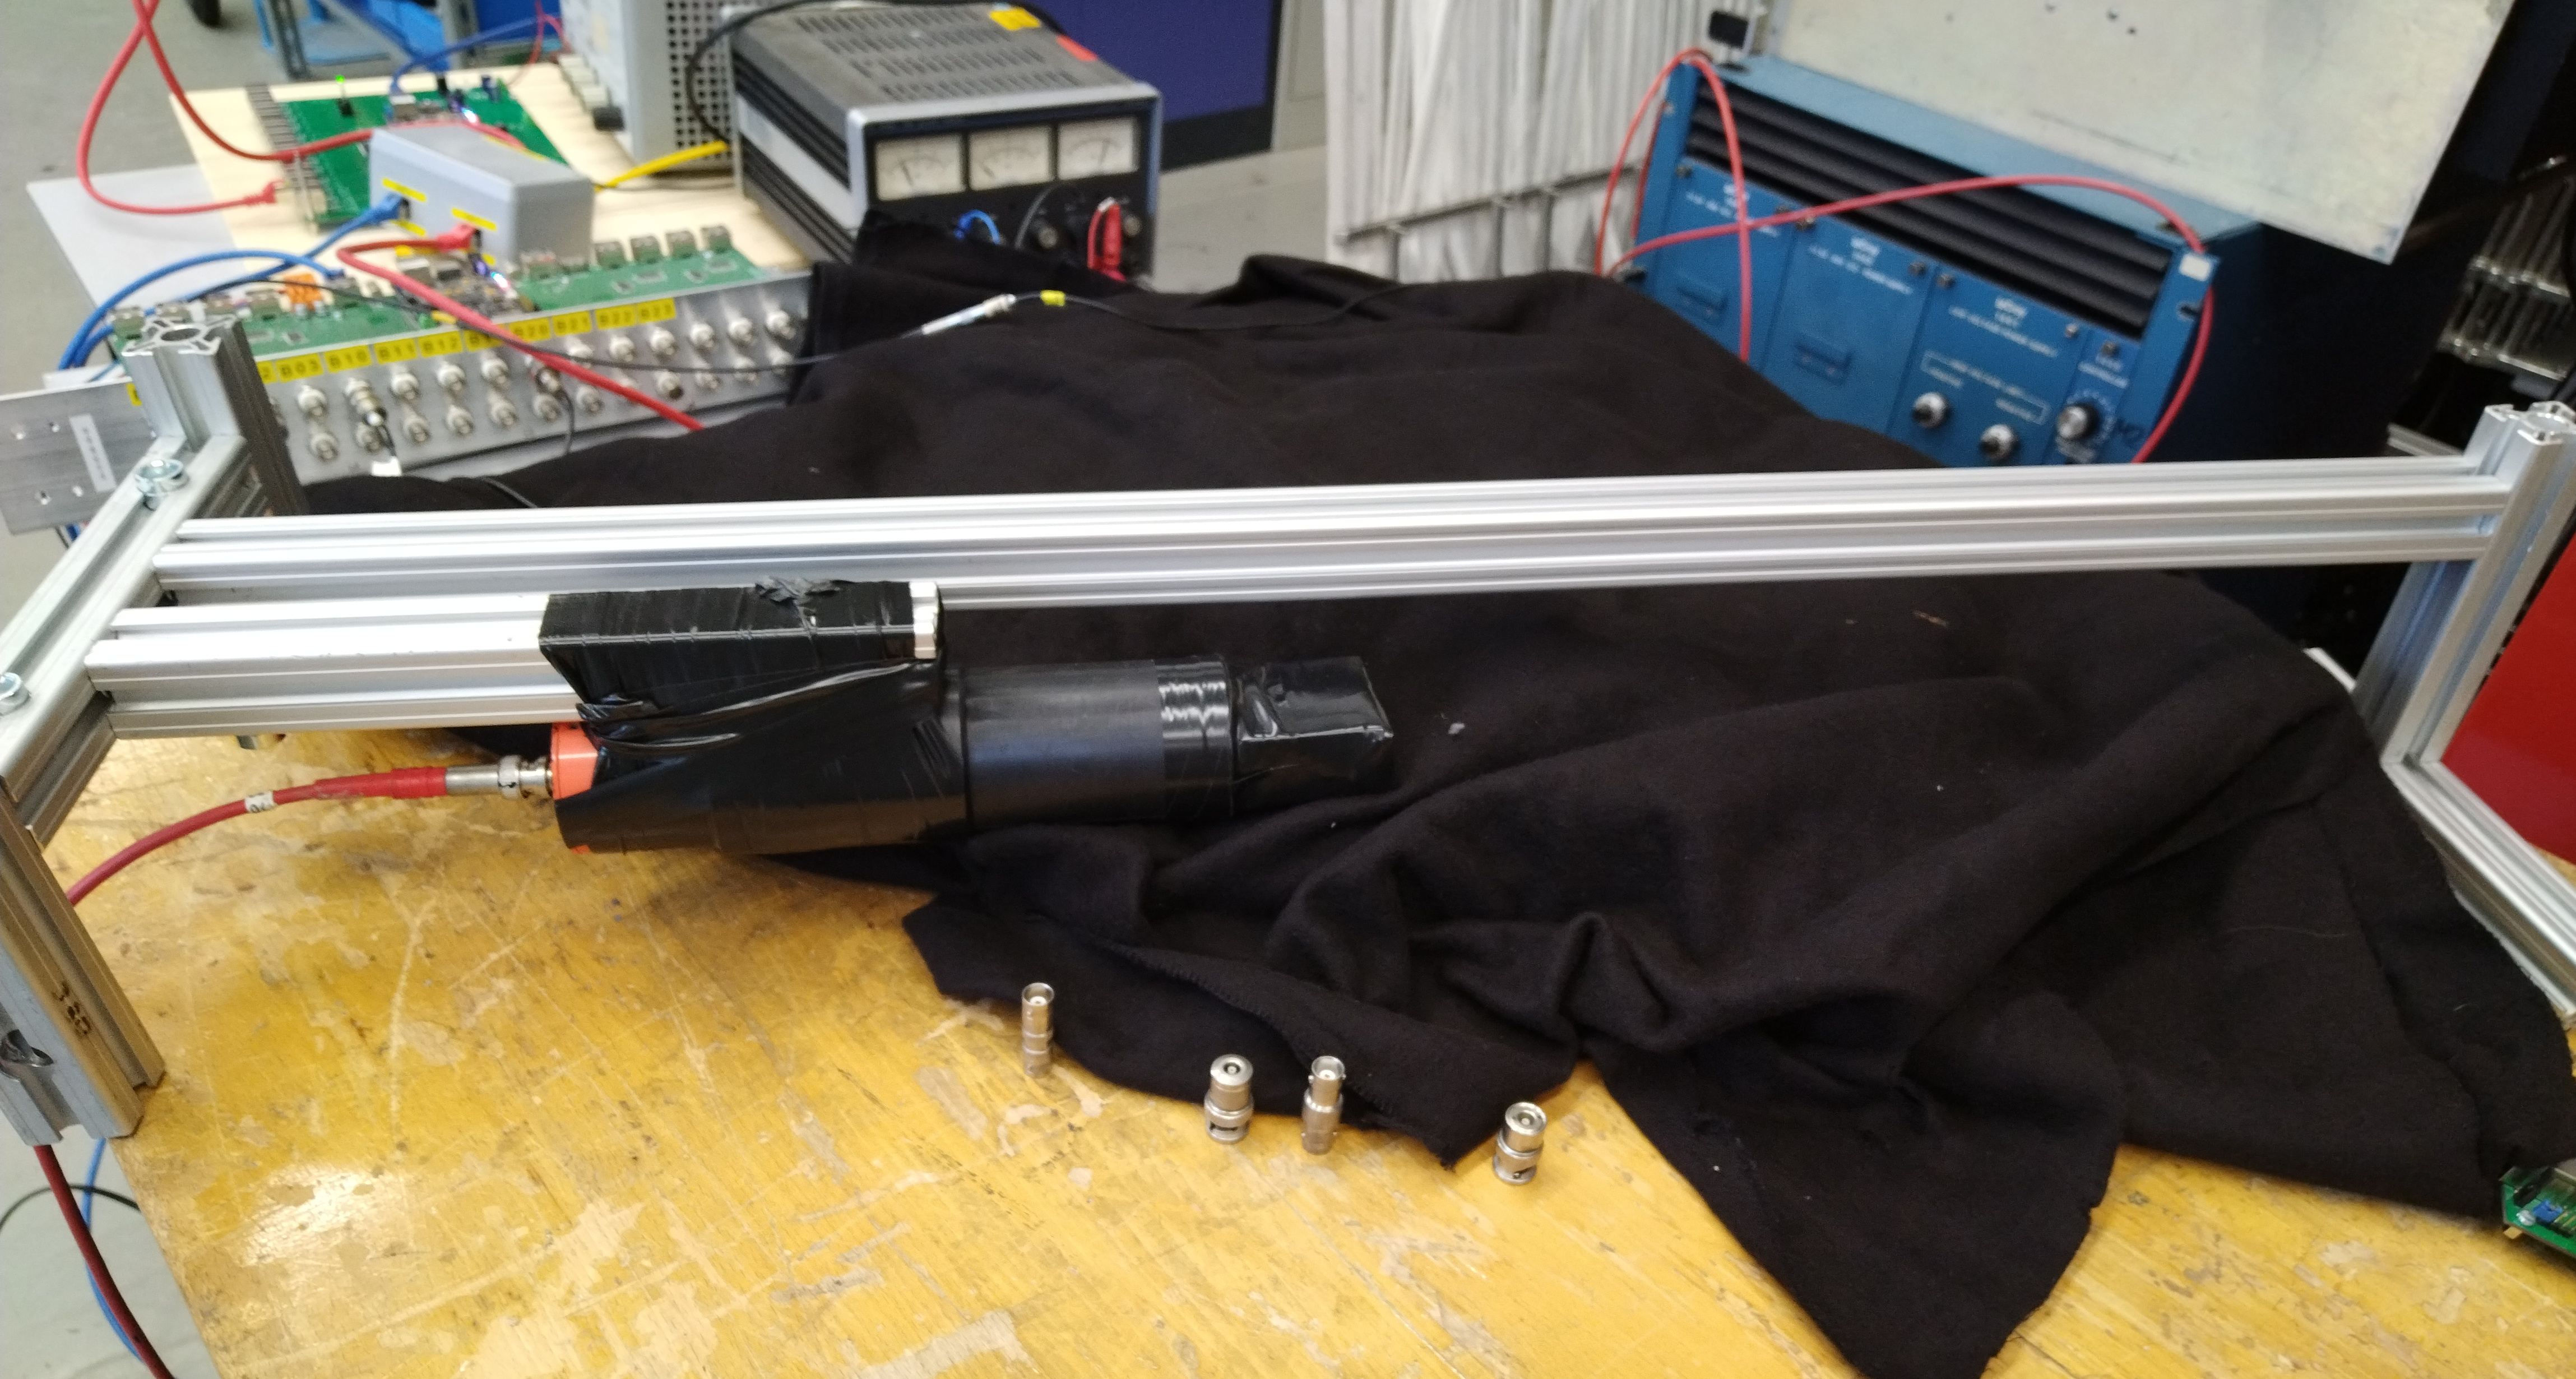
\includegraphics[width = 0.5\textwidth]{figures/IMG_20221107_152816.jpg} 
\caption{Setup to study the correlation between the pmts, the detector B was covered by a black blanket to shield the detector from optical photons.}
\end{figure}
\begin{center}
\begin{tabular}{|c|c|c|c|c|}
\hline 
 & pmt0 & pmt1 & pmt2 & pmt in coincidence \\ 
\hline 
1 & 63 & 57 & 72 & 28 \\ 
\hline 
2 & 55 & 51 & 64 & 18 \\ 
\hline 
3 & 62 & 53 & 75 & 27 \\ 
\hline 
4 & 71 & 62 & 75 & 33 \\ 
\hline 
5 & 68 & 59 & 49 & 23 \\ 
\hline 
6 & 57 & 55 & 63 & 18 \\ 
\hline 
7 & 70 & 64 & 64 & 24 \\ 
\hline 
8 & 50 & 69 & 69 & 25 \\ 
\hline 
9 & 65 & 62 & 62 & 19 \\ 
\hline 
10 & 74 & 71 & 77 & 28 \\ 
\hline 

\end{tabular} 
\end{center}

\begin{equation*}
\begin{split}
\mu_{0} = 63.5 \qquad \sigma^{2} = 58.9 \qquad r_{3} = 0.65 \\
\mu_{1} = 60.3 \qquad \sigma^{2} = 43.3 \qquad r_{2} = 0.38 \\
\mu_{2} = 67.0 \qquad \sigma^{2} = 71.1 \qquad r_{1} = 0.49 \\
\end{split}
\end{equation*}

The results are fine, we are able to see a positive correlation between the counts of the pmts in coincidence, and it is proof that the threshold, the voltage and attenuation were correclty set.
The same procedures of calibration were performed on the Detector A,too. It is made by 9 pmts (but only 8 of them will be used for experiment). For the pmts 6,7,8,9 we finally selected a voltage of $\SI{-1050}{\volt}, \SI{-1086}{\volt}, \SI{-950}{\volt}, \SI{-1050}{\volt} $ and an attenuation of $575$ for all the four pmts:

\begin{figure}[hbtp]
\centering
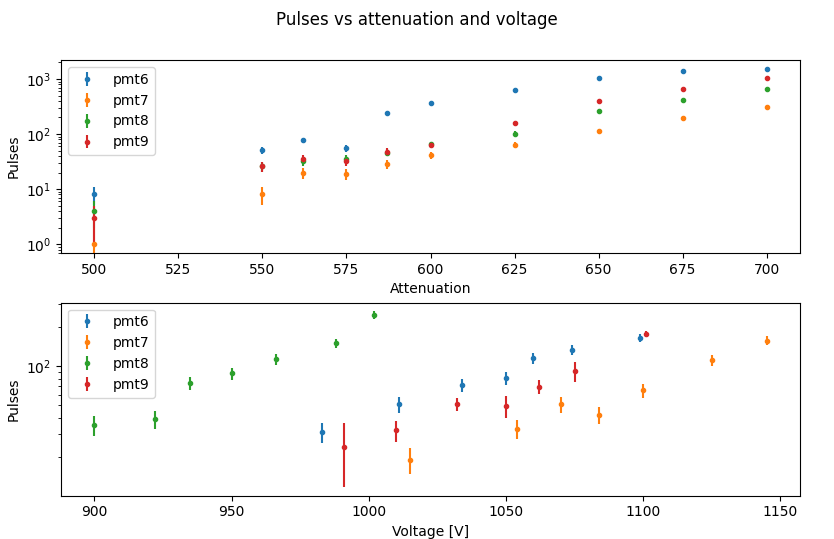
\includegraphics[width= 0.5\textwidth]{figures/AttenuationA6789.png}
\caption{•}
\end{figure}


For the last 4 pmt used for the detector A, we raised the power of the pmt 4,3,2 down to $\SI{-1450}{\volt}$, and for 5 pmt to \SI{-1000}{\volt} in order to see some signals. Then we raised the threshold in the daq program up to 1000, and we tried to see some coincidence, with an attenuation of 750,725,775 for the pmt 4 3 2, (the pmt number 5 was not included, since we need one power supply for the pmt in coincidence). 
\begin{center}
\begin{tabular}{|c|c|c|c|c|}
\hline 
pmt & 4 & 3 & 2 & pmt in coincidence \\ 
\hline 
1 & 91 & 51 & 50 & 27 \\ 
\hline 
2 & 86 & 61 & 50 & 7 \\ 
\hline 
3 & 58 & 48 & 45 & 18 \\ 
\hline 
4 & 95 & 62 & 41 & 29 \\ 
\hline 
5 & 69 & 60 & 50 & 21 \\ 
\hline 
6 & 85 & 57 & 45 & 19 \\ 
\hline 
7 & 66 & 51 & 46 & 28 \\ 
\hline 
8 & 74 & 51 & 48 & 22 \\ 
\hline 
9 & 77 & 43 & 45 & 17 \\ 
\hline 
10 & 62 & 44 & 50 & 29 \\ 
\hline 
\end{tabular} 
\end{center}

\begin{equation*}
\begin{split}
\mu_{4} = 76 \qquad \sigma^{2} =160  \\
\mu_{3} = 52.7 \qquad \sigma^{2} = 49.8 \\
\mu_{2} = 47  \qquad \sigma^{2} = 9.6
\end{split}
\end{equation*}

This data are not what we expect, observing that for the other Detector we were able to see strong correlation with the sigle pmt in coincidence. Furthemore the variance of the counts is very different from the variance we expect from a poisson distribution. We decided to move the attenuation for the pmt 4,3,2 to the following values: 700 700 725 and take other 10 counts, one minute long, to see if the working point is better than before.


\begin{center}
\begin{tabular}{|c|c|c|c|c|}
\hline 
pmt & 4 & 3 & 2 & pmt in coincidence \\ 
\hline 
1 & 43  & 36 & 30 & 13 \\ 
\hline 
2 & 56 & 30 & 46 & 17 \\ 
\hline 
3 & 49 & 42 & 35 & 23 \\ 
\hline 
4 & 34 & 27 & 33 & 16 \\ 
\hline 
5 & 60 & 38 & 49 & 19 \\ 
\hline 
6 & 54 & 44 & 38 & 20 \\ 
\hline 
7 & 54 & 42 & 36 & 17 \\ 
\hline 
8 & 47 & 44 & 51 & 16 \\ 
\hline 
9 & 48 & 41 & 43 & 14 \\ 
\hline 
10 & 49 & 39 & 31 & 16 \\ 
\hline 
\end{tabular} 
\end{center}

\begin{equation*}
\begin{split}
\mu_{4} = 53.8 \qquad \sigma^{2} = 49.4 \qquad  r_{4} = 0.41 \\
\mu_{3} = 33.6 \qquad \sigma^{2} = 38.3 \qquad r_{3} = 0.29 \\
\mu_{2} = 57.28  \qquad \sigma^{2} = 39.2 \qquad r_{2} = 0.09 \\
\end{split}
\end{equation*}

Now the pmt 4 and 3 seems to be in the correct values for threshold, attenuation and power. The last pmt has a variance less than the expected, and don't seem to be correlated with the other pmt. We decided to put the pmt in coincidence near to the second pmt, and raise the attenuation for the pmt number two, so now the attenuation is set to: 700,700,750 (725 coincidence, before 700).

\begin{center}
\begin{tabular}{|c|c|c|c|c|}
\hline 
pmt & 4 & 3 & 2 & pmt in coincidence \\ 
\hline 
1 & 49  & 39 & 31 & 10 \\ 
\hline 
2 & 61 & 40 & 41 & 20 \\ 
\hline 
3 & 64 & 48 & 32 & 11 \\ 
\hline 
4 & 82 & 36 & 49 & 20 \\ 
\hline 
5 & 64 & 38 & 35 & 21 \\ 
\hline 
6 & 42 & 41 & 39 & 15 \\ 
\hline 
7 & 73 & 36 & 36 & 21 \\ 
\hline 
8 & 60 & 35 & 42 & 21 \\ 
\hline 
9 & 54 & 36 & 40 & 21 \\ 
\hline 
10 & 63 & 35 & 36 & 16 \\ 
\hline 
\end{tabular} 
\end{center}

Now we report the mean count, the variance and the correlation between the pmt number two and the pmt in coincidence:

\begin{equation*}
\mu_{2} = 38.1 \qquad \sigma^{2} = 28.1 \qquad r_{2} = 0.63
\end{equation*}

The correlation is positive and high, so the behaviour of the pmt 2 seems correct, now. But for the pmt 4 and 3 we observed:

\begin{equation*}
\begin{split}
\mu_{4} = 61.2 \qquad \sigma^{2} = 129 \\
\mu_{3} = 38.4 \qquad \sigma^{2} = 15.8 \\
\mu_{C} = 17.6 \qquad \sigma^{2} = 18.7 \\
\end{split} 
\end{equation*}

Here we see that the variance of the pmt 4 in roughly 2 times what we expect, while for the pmt 3 it is the half. This is quite surprising because all the values of the Detector A were fixed to the same values of the previous 10 runs, where the counts were in agreement with what we expect. Due to this strange behavior, we will focus our attention on calibrating the last four pmt, during the first day of the beam time, using directly the counts from the scattered electron.

Now we took some runs with pmt number 5

\begin{center}
\begin{tabular}{|c|c|c|c|c|c|c|c|c|c|c|}
\hline 
pmt 5 & 47 & 60 & 59 & 60 & 61 & 71 & 60 & 86 & 68 & 83 \\ 
\hline
pmt in coincidence & 16 & 17 & 17 & 16 & 21 & 14 & 17 & 19 & 12 & 23 \\ 
\hline 
\end{tabular} 
\end{center}

The result are 

\begin{equation*}
\mu_{5} = 65 \qquad \sigma^{2} = 128.6  \qquad \mu_{C} = 17 \qquad \sigma^{2} = 7.2 \qquad r = 0.29\\
\end{equation*}

For the last pmts of detectorA, we observe some differences from the expected behaviour. For the beam time, we will focus our attention on calibrating the last four pmt, carefully.\newline
Now we report a table with all the final values of settings:

\begin{center}
\begin{tabular}{|c|c|c|c|}
\hline 
\textbf{detector B} & pmt 1 & pmt 2 & pmt 3 \\ 
\hline 
Voltage & \SI{-951}{\volt} & \SI{-925}{\volt} & \SI{-918}{\volt} \\ 
\hline 
attenuation & 600 & 600 & 600 \\ 
\hline 
threshold & 600 & 600 & 600 \\ 
\hline 
\end{tabular} 
\end{center}

\begin{tabular}{|c|c|c|c|c|c|c|c|c|}
\hline 
\textbf{Detector A} & pmt 2 & pmt 3 & pmt 4 & pmt 5 & pmt 6 & pmt 7 & pmt 8 & pmt9 \\ 
\hline 
Voltage & \SI{-1450}{\volt} & \SI{-1450}{\volt} & \SI{-1450}{\volt} & \SI{-1000}{\volt} & \SI{-1050}{\volt} & \SI{-1086}{\volt} & \SI{-950}{\volt} & \SI{-1050}{\volt} \\ 
\hline 
attenuation & 750 & 700 & 700 & 700 & 575 & 575 & 575 & 575 \\ 
\hline 
threshold & 1000 & 1000 & 1000 & 1000 & 600 & 600 & 600 & 600  \\ 
\hline 
\end{tabular} 


\section{Analysis.cc}

This is the main part of the Analysis program, where the data tree is filled and txt files with the data are produced for the fit.cc script, that will extract with the desired regresssion the parameters from the data. The program parses the RunData from the data acquisition board and start filling the \textit{Data-tree}. With the script \textit{HistosVoltage.cc} it's possible to create and fill some histograms, using the gnuplot library. At the beginning the program loads all the useful quantities stored in the \textit{standard.conf} file, then it fill the data tree with the rawValues (VFC counts) for the monitors and the two detectors. After this, the program fills all the other values needed for the analysis, with the functions defined in the scripts \textit{Calculation.cc}. Then the program calculate useful statistics for the \textit{MomentumMethod.py} script, for a first estimation of the parameters.


following part still in italian, deprecated 
\begin{comment}

\subsection{MomentumMethod.py TODO}
Questo scripts serve ad estrarre i parametri dal file txt \textit{filename+stats}. AL programma si deve passare da riga di comando il nome del file senza il \textit{txt} alla fine, - seguito da quali su cui eseguire l'analisi (-XY farà l'analisi sull'asimmetria in funzione della posizione), in seguito si deve indicare il numero di variabili indipendenti (-number). A quel punto il programma esegue l'analisi richiesta.


\section{Histogram}

\subsection{CleverHisto.cc}

In questo script è definita la funzione principale che riempie gli istogrammi. Gli istogrammi sono numerati con un indice e sono identificati tramite la funzione CleverHisto::identify(string identifier)
che compara il titolo dell'istogramma e permette così di riempirlo. La struttura che contiene tutti i parametri dell'istogramma è definita in \textit{CleverHisto.h}. 

\subsection{SimpleHisto.cc}

Qui è definita la struttura base di un istogramma, che viene riempito richiamando la funzione fill di cleverhisto. Alcuni variabili importanti sono myBins, myMinimum, myMaximum. MyBins è il numero di bins dell'istogramma, myMinimum e myMaximum sono gli estremi dell'istogramma. La funzione SimpleHisto-fill prende in input il valore da inserire, calcola il bin corrispettivo come (myBins) * (value - myMinimum) / (myMaximum - myMinimum) e aggiorna i conteggi in data[bin].

Qui viene riportato lo schema per riempire un istogramma:
\begin{itemize}
\item Nell'event-loop in Analysis.cc si chiama la funzione -fillHistograms(0), della classe \textit{HistoDefinition}
\item in \textit{HistoDefinition} è definita la funzione fill, che richiama il file \textit{HistosVoltage.cc} dove sono definiti tutti gli istogrammi da riempire (nel file vale la sostituzione "define HISTOGRAM  myCleverHisto-fill")
\item quindi la funzione fill() di \textit{CleverHisto.cc} è chiamata. Questa prende in input tanti paramentri come nome dell'istogramma, numero bin... la funzione come prima cosa definisce una serie di variabili tra cui un SimpleHisto che poi verrà riempito 
\item 
\end{itemize}

\section{RunParser.cc}

In questo script si estraggono i dati dal file dati e si riempie la struttura ad albero. Il programma legge gli header del file, che indicano alcune inforzioni sul tipo di evento, e poi i vari data-packages, che possono essere pacchetto dati, pacchetto beam, o altri pacchetti riguardanti lo stato dell'elettronica. Il programma legge prima i file header e poi i pacchetti, che sono in formato esadecimale. 

\subsection{MomentumMethod.py}
Questo programma serve ad estrarre i parametri dal file txt \textit{filename+stats}. AL programma si deve passare da riga di comando il nome del file senza il \textit{txt} alla fine, - seguito da quali su cui eseguire l'analisi (-XY farà l'analisi sull'asimmetria in funzione della posizione), in seguito si deve indicare il numero di variabili indipendenti (-number). A quel punto il programma esegue l'analisi richiesta.
\end{comment}
\end{document}